\documentclass{article}

\usepackage{amsmath}
% 312 Font
\usepackage{charter}
% Custom lists
\usepackage{enumitem}
% Page margins & pagestyles
\usepackage{fullpage}
% Font encoding
\usepackage[T1]{fontenc}
% Colored boxes around the 'solution' environment
\usepackage{mdframed}
% Used for making FSMs
\usepackage{tikz}
\usetikzlibrary{automata, positioning}
% For color
\usepackage[dvipsnames]{xcolor}

% Defines a solution environment that creates a green box around text inside.
\mdfdefinestyle{SolutionFrame}{linecolor=green!60!black,linewidth=1pt}
\newenvironment{solution}{\begin{mdframed}[style=SolutionFrame]}{\end{mdframed}}

% Enumerate with (a),(b),(c),...
\newenvironment{enum}{\begin{enumerate}[label={(\alph*)}]}{\end{enumerate}}

% Put a dot after section titles
\renewcommand\thesection{\arabic{section}.}
\renewcommand\thesubsection{\arabic{section}.\arabic{subsection}.}

% Tikz styles & configs
\tikzset{
    node distance=2cm,
    initial text=$ $,
}

% Images {img_size = 1.0, file_path}
\newcommand{\img}[2][1.0]{
    \begin{minipage}[t]{\linewidth}
        \begin{center}
            \includegraphics[width=#1\linewidth]{#2}
        \end{center}
    \end{minipage}
}

% Hide the Date
\date{}
% Hide page numbers
\pagenumbering{gobble}

\begin{document}
    \begin{titlepage}
        \centering
        \null
        \vspace{5cm}
        {\Huge CSE 369 Lab 8\par}
        \vspace{0.5cm}
        {\Large Final Project: DDR \par}
        \vfill
        {\hfill \Large Isaac Wu \par}
        {\hfill \large 2360957 \par}
        {\hfill \large \today \par}
    \end{titlepage}

\section{Instructions}
    \begin{solution}
        Once programmed, flip SW0 to reset the game to guarantee correct behavior. Then, on the LED Board, red notes will `fall' from the top of the board to the bottom. There is a row of orange lights, which represent the hit zone. Your note inputs are the KEY buttons and your goal is to press the corresponding button when a note overlaps with the hit zone row. \\
        If you press the input at the correct time, the hit zone light will turn green, and will be red otherwise. If you hit at the right time, then two points will be added to your score. If you are one row early, then you will get one point. If you are more than two rows early or just press an input when there is no note present, then two points will be deducted from your score. You can hold down a button to repeatedly press each clock cycle if there is a large column of notes in one track.
    \end{solution}

\section{Top-Level Block Diagram}
    \begin{solution}
        \img{block_diagram.png} \\

        \newpage
        This is my Top-Level Block Diagram for the DDR module. This module takes in 5 inputs, KEYs 0-3 as input presses, and SW0 as a Reset switch. I chose not to synchronize the KEY inputs because it would introduce too much delay between when KEYs were pressed and when they were registered in the system. I also chose not to use an Edge Detector to make it easier for Users to hit multiple notes in a row.

        I split each column of notes into their own separate Track module. Each track gets its own KEY as user input, and a `note' input that instructs the module to create a new `note' at the start of its range. The Track modules keep its state as if they were handling rows for simpler handling. At each rising clock edge, the track will shift its contents leftward. The track will keep track of when the input is registered and will reward or deduct points according to how accurate the input was to the note's position.

        I used the exact same 9-Bit LFSR from Lab 7 as a randomizer. I took two bits from its resulting status each cycle and \&'d them together and passed it into each Track's note input. Track 0: [6] \& [3], Track 1: [2] \& [5], Track 2: [4] \& [8], Track 3: [7] \& [1].

        The light statuses from each Track module is combined together and then passed through a Transpose module to convert the rows of lights the Tracks keep track of into columns of notes to display. The resulting light matrices are then passed to the provided LED Driver (along with the reset input), which controls the connected LED Board through the GPIO\_1 output.

        The points from each track is passed to a Point Adder module, which calculates the total amount of points earned/lost this cycle. This total is passed into a chain of Digit modules.
        
        Each Digit module takes in a current state representing the digit that is currently being displayed (coming from the Digit Display module) and an input to add to the current total. This module is responsible for handling all of the overflow/underflow that occurs when the result is greater than 10 or negative. The resulting state is given to a matching Digit Display module. These modules simply keep track of their current state and outputs to a HEX display, which shows its state as a number between 0-9. The carry outputs from the Digit modules are passed down the chain as their inputs.
    \end{solution}

\newpage
\section{Top-Level Simulation}
    \begin{solution}
        Red \& Green rows are shown in hex here, and KEYs are 1s by default and the input handling takes the inverse. \\
        \img{DDR_start_waves.png}
        This is the behavior of the top-level module right after a reset input at the beginning. Notes take a few cycles to start appearing and moving down the tracks. \\
        \img{DDR_end_waves.png}
        Here, KEYs are pressed on time when notes are at the hit zone, updating the scores displayed on the HEXs.
    \end{solution}

\newpage
\section{Track Module}
\subsection{Finite State Machine}
    \begin{solution}
        \begin{center}
        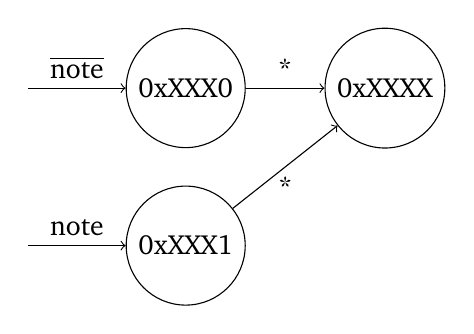
\begin{tikzpicture}
            \node[state] (0) {0xXXX0};
            \node[state, below of=0] (1) {0xXXX1};
            \node[state, right=1cm of 0] (x) {0xXXXX};

            \path
                (0) ++(-2,0) edge[->] node[above] {$\overline{\text{note}}$} (0)
                (1) ++(-2,0) edge[->] node[above] {note} (1)
                (0) edge[->] node[above] {*} (x)
                (1) edge[->] node[below] {*} (x)
            ;
        \end{tikzpicture}
        \end{center}
        I am not entirely sure what the correct method is for making this FSM. If I were to draw it accurately it would have 65,536 states and way too many transitions. The Track module uses a [15:0] buffer that adds a note if it is input at the end and shifts its data to the left after each clock cycle.
    \end{solution}
\subsection{Simulation}
    \begin{solution}
        \img{track_waves.png}
        I reset the module at the beginning. Then, I input two note inputs to create two new notes. You can see them appear on row 0 of the red matrix one clock cycle afterwards. The red and grn matrices are displayed in this diagram as a collection of rows represented in hex. These notes move up one row after each clock cycle. Some time after, I enter an erroneous user input to simulate miss behavior. This results in the green LEDs in the hit zone turning off to show red lights in that row and a Miss encoding in the point output (00). When no input is being pressed, the point output changes to Idle (01). After some more time, an input is pressed one row too early (as seen, row 14 is the hit zone and at this cycle, the note is on row 13), resulting in Early points (10). Then, the input is pressed right when the note is on row 14. This results in the red light in the hit zone row turning off to display green. The points output also changes to a Hit (11). Notice that on the next clock cycle, the hit note does not continue on to row 15.
    \end{solution}

\newpage
\section{Point Adder Module}
    \begin{solution}
        \img{point_adder_waves.png}
        In this test bench, I demonstrate the proper decoding from the input to their correlated points. As a reminder, 00 means a Miss (-2 points), 01 is Early (+1 points), 11 is a Hit (+2 points), and 10 is Idle (0 points). This module just takes each input in pts and adds them together. The total output is displayed as a signed integer.
    \end{solution}

\section{Digit Module}
    \begin{solution}
        \img{digit_waves.png}
        This module takes the current state, adds the input, and outputs the corresponding digit and any carry outputs. The current state and output state is displayed as an unsigned integer (since the digit state is between 0 and 9). The input is displayed as a signed decimal (because the point total can be as low as -8 and as high as 8). The carry is also displayed as signed. This test bench demonstrates when the current state is 0, overflow, and underflow.
    \end{solution}

\newpage
\section{Digit Display Module}
\subsection{Finite State Machine}
    \begin{solution}
        \begin{center}
        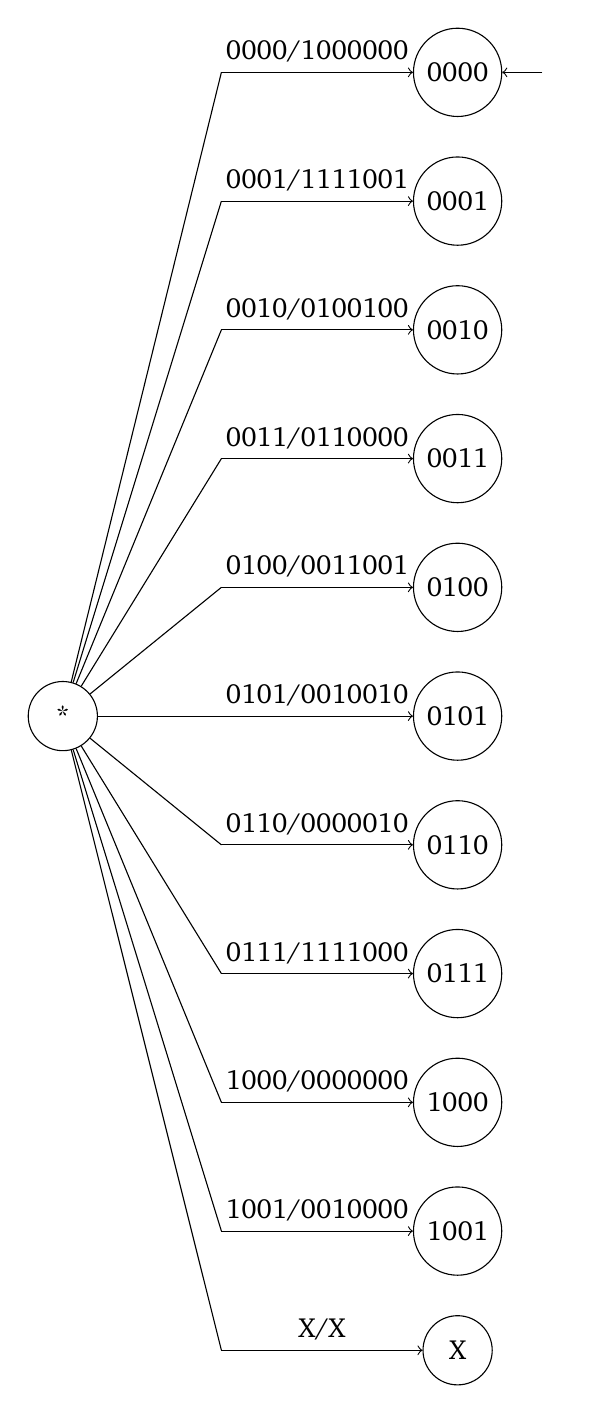
\begin{tikzpicture}
            \node[state] (*) {*};

            \node[state, right=4cm of *] (0101) {0101};
            \node[state, above=.5cm of 0101] (0100) {0100};
            \node[state, above=.5cm of 0100] (0011) {0011};
            \node[state, above=.5cm of 0011] (0010) {0010};
            \node[state, above=.5cm of 0010] (0001) {0001};
            \node[state, above=.5cm of 0001, initial, initial where=right] (0000) {0000};
            \node[state, below=.5cm of 0101] (0110) {0110};
            \node[state, below=.5cm of 0110] (0111) {0111};
            \node[state, below=.5cm of 0111] (1000) {1000};
            \node[state, below=.5cm of 1000] (1001) {1001};
            \node[state, below=.5cm of 1001] (X) {X};

            \coordinate (s0000) at ([shift={(-3,0)}]0000);
            \coordinate (s0001) at ([shift={(-3,0)}]0001);
            \coordinate (s0010) at ([shift={(-3,0)}]0010);
            \coordinate (s0011) at ([shift={(-3,0)}]0011);
            \coordinate (s0100) at ([shift={(-3,0)}]0100);
            \coordinate (s0101) at ([shift={(-3,0)}]0101);
            \coordinate (s0110) at ([shift={(-3,0)}]0110);
            \coordinate (s0111) at ([shift={(-3,0)}]0111);
            \coordinate (s1000) at ([shift={(-3,0)}]1000);
            \coordinate (s1001) at ([shift={(-3,0)}]1001);
            \coordinate (sX) at ([shift={(-3,0)}]X);
            
            \path
                (s0000) edge[->] node[above] {0000/1000000} (0000)
                (s0001) edge[->] node[above] {0001/1111001} (0001)
                (s0010) edge[->] node[above] {0010/0100100} (0010)
                (s0011) edge[->] node[above] {0011/0110000} (0011)
                (s0100) edge[->] node[above] {0100/0011001} (0100)
                (s0101) edge[->] node[above] {0101/0010010} (0101)
                (s0110) edge[->] node[above] {0110/0000010} (0110)
                (s0111) edge[->] node[above] {0111/1111000} (0111)
                (s1000) edge[->] node[above] {1000/0000000} (1000)
                (s1001) edge[->] node[above] {1001/0010000} (1001)
                (sX) edge[->] node[above] {X/X} (X)
            ;
            
            \draw (*) -- (s0000);
            \draw (*) -- (s0001);
            \draw (*) -- (s0010);
            \draw (*) -- (s0011);
            \draw (*) -- (s0100);
            \draw (*) -- (s0101);
            \draw (*) -- (s0110);
            \draw (*) -- (s0111);
            \draw (*) -- (s1000);
            \draw (*) -- (s1001);
            \draw (*) -- (sX);
        \end{tikzpicture}
        \end{center}
        The * state represents any state. In this module, no matter the present state, the next state is dependent only on its input. The output is the HEX display for that digit, which is defined for digits 0000 to 1001, and is undefined for digits 1010 to 1111.
    \end{solution}

\newpage
\subsection{Simulation}
    \begin{solution}
        \img{digit_display_waves.png}
        This simple test bench first resets the module, then increments the input state to 10. One clock cycle after the input changes, the HEX output switches to display the state and its state is output accordingly.
    \end{solution}

\section{Transpose Module}
    \begin{solution}
        \img{transpose_waves.png}
        The matrices in this diagram are displayed in hexadecimal. In this test bench, I set two rows of the input module, 0 and 13, to all 1's. The output shows the equivalent transposed matrix, with columns 0 and 13 set to all 1's, represented by each row in the output being 0x2001.
    \end{solution}

\section{Testing}
    \begin{solution}
        My method for testing my project was to test each module individually before combining them together. For example, the Digit modules I created had to be re-made three times to organize how the base 10 overflow was being handled, the HEX display output was being updated, and what module was keeping track of the internal state of the digit. Then, testing the carry output chaining into the other digit modules had to be tested as a group, and only after that could I be confident my Digit module was sufficient enough to use in my top-level module.
    \end{solution}

\section{Misc.}
    How many hours (estimated) it took to complete this lab in total, including reading, planning, designing, coding, debugging, and testing.
    \begin{solution}
        It took around 26 hours in total to complete this lab.
    \end{solution}

\end{document}